\documentclass[12pt]{report}
\usepackage{titlesec}


\usepackage{geometry}
\geometry{
	a4paper,
	total={210mm,297mm},
	left=40mm,
	right=10mm,
	bottom=20mm,
	top=20mm,
}


\usepackage{setspace}
\usepackage{graphicx}
\usepackage{natbib}
\bibliographystyle{abbrvnat}
\setcitestyle{authoryear,open={(},close={)}}
\doublespacing
\begin{document}
	\begin{titlepage}
		\centering
		\vspace*{0.5 cm}
		
\includegraphics[scale=0.75]{nust.png}	% University Logo
		\begin{center}    \textsc{\Large   NATIONAL UNIVERSITY OF SCIENCE AND TECHNOLOGY}\\[2.0 cm]	\end{center}% University Name
		\textsc{\Large 2019  }\\[0.5 cm]				% Course Code
		\rule{\linewidth}{0.2 mm} \\[0.4 cm] 
		Project Title: Sentiment Analysis for Library.
		\rule{\linewidth}{0.2 mm} \\[1.5 cm]
		
		
		Faculty : Applied Sciences 
		
		
		Department :Computer Science (Conv) 
		
		
		Student Name: Howard Mabhugu
		
		Student Number: N0161388M
		
		Supervisor : Mr D. Musundire
		
		
		
		\null
		\null
		\null
		\null
		\null
		\null
		\null
		\textit{This proposal document is submitted in partial fulfilment of the requirements of the BSc (Hons) Computer Science at the National University of Science  and Technology.}
		
	\end{titlepage}
	
	\tableofcontents
	
	\chapter{Introduction}
	\section{Introduction}
	Computational intelligence methods are proving to be valuable strategic tools in many industries with the increasing popularity of analytics and data science \cite{yang2016social}. For instance, data is mined for patterns in business analytics that would help better understand customers and improve sales and marketing. Methods of computational intelligence make it possible to use probabilistic methods to find patterns in data. Typically, these methods work on low-level data and are not guided by absolute knowledge, as with general artificial Intelligence methods. In addition, a huge amount of data is now generated in written form which warrants analysis. The written text is subject to interpretation, and it is difficult to represent the data in an absolute syntax (such as a binary system). Computational intelligence methods, however, require such fluidity and may be the most appropriate methods to find trends in such data, hence sentiment analysis comes in.\\
	According to Oxford Sentiment analysis is the process of computationally identifying and categorizing opinions expressed in a piece of text, especially in order to determine whether the writer's attitude towards a particular topic, product, etc. is negative, positive, or neutral. This subject brings together various research areas such as natural language processing, data mining and text mining, and is rapidly becoming of major importance to organizations as they strive to integrate computational intelligence methods into their operations and attempt to shed more light on their products and services and improve them. Sentiments are opinions or views about a certain object. This concept can be applied in different areas that includes marketing, social media monitoring, brand monitoring, customer feedback, customer service.\\
	Sentiment analysis can be applied in libraries. A library is a collection of resources in a variety of formats that is (1) organized by information professionals or other experts who (2) provide convenient physical, digital, bibliographic, or intellectual access and (3) offer targeted services and programs (4) with the mission of educating, informing, or entertaining a variety of audiences (5) and the goal of stimulating individual learning and advancing society as a whole \citep{eberhart2010librarian}. Libraries are key elements of a healthy community so they are vital in a society. To maintain their vitality to the society they need to be maintained based on customers’ view. Thereby incorporating sentiment analysis will help in easily visualising the view of customers on the resources in a library.
		
	\section{Background}
	Sentiment analysis is a new computational intelligence subject that has a number of researches in different fields that ranges from management science to computer science, social science and business \cite{alessia2015approaches}. A number of researches were done with the aim of trying to apply this concept to different areas.\\ 
	Sentiment analysis has been applied in hotel systems \citep{yang2016social}. \cite{yang2016social} used sentiments from TripAdvisor with the aim of proving that machine learning techniques of analysing sentiments are better than human produced sentiments. The output proved that machine language is faster, thus it saves time and saves cost to hotels.\\
	In the entertainment industries sentiments researches where done on its application to platform such as YouTube. \cite{asghar2015sentiment} did a research on the application of Sentiment analysis to YouTube. A number of challenges where met that include failure to analyse different languages that YouTube customer comments with.\\ 
	\cite{bogicevic2013airport} also did a research about application of sentiment analysis in airports. The research was mainly targeted to see the view of customers on the services offered by the airport and see which services are distractors and which one are enhancers of customers travel on the airport. This is application of sentiment analysis in the field of customer satisfaction.\\
	Customer involvement in the day to day operation of any firm is of uttermost important and sentiment analysis makes this process easier. Sentiment analysis let the voice of customers be heard out. So it brings advantages to the customers of letting them complains be heard and at the same time it helps organisations to maintain their market share since customers will remain loyal to an organisation that listen to their objectives. Sentient analysis brings a market advantage to affirm that uses it.\\
	The application of sentiment analysis to libraries is also an avenue that remains unexploited. With the introduction of Library 2.0 there is need for interacting with the customers to see their view to information contained in the library and help the library owner with decision making.\\
		
	\section{Problem Statement}
	The web has created jobs for a number of people through video sharing, article writing, and music uploading, this calls the need for library owners to understand what viewers of the resources in the libraries are saying so as to maintain market share. Viewing every comment left by the resource viewers is tedious and time consuming, and there is no system that helps with viewing the comments and visualise them for the library owner. 
	\section{Aim}
	Designing a model that does sentiments mining from library comments.
	\section{Objectives}
	\begin{enumerate}
				
		\item To train the Support Vector Machine Algorithm.
		\item To allow patrons to leave feedback in the system anonymously.
		\item To omit noisy feedback / data during analysis.
		\item  Classify the comments from patrons into positive negative and neutral, to help in feedback review using Support Vector Machine Algorithm.
		\item To generate periodic reports of analysed information using line graph and pie chart.
		\item Highlight negative feedback to Video library owners.
				
	\end{enumerate}
	
	
	\section{Justification}
	There is a number of valid reasons why this system must be produced. The reasons include allowing customers to comment to a resource, reduction of task overload on the library owner and alert on customer dissatisfaction on library resources.\\
	Firstly, the sentiment analysis system for libraries helps in evaluating the extent to which customers are satisfied by the resources offered in a library. This is achieved through the use of a commenting section where customers drop their comments on the resources they are receiving expressing their view and feelings.\\
	In addition, the system will help libraries owners by alerting them about customers’ dissatisfaction before it is worse. The system will visualize the sentiments reports of every month so that the library owner sees the satisfaction rate of customers. Basing on the reports the library owner decides the necessary actions that will help maintain the market share or keep the customers satisfied on the next resource that will be uploaded.\\
	Lastly, sentiment analysis saves time of going through each and every comment that customers leave one by one. The system will analyse the comments and produce a report that summarise the comments from patrons instead of library owner analysing the comments on their own.
	
	\section{Methodology}
	In this project Cross-Industry Standard Process for Data Mining (CRISP-DM) methodology is going to be adopted. CRISP DM is a methodology that is applied much in data mining but it is considered to be a standard methodology applied to the extraction of knowledge from big data sets \citep{sharda2016business}. Sentiment analysis works with datasets for training of systems either training the system using supervised learning algorithms or unsupervised learning algorithm. Not every step that the CRISP-DM is going to be used, so the methodology will be twisted a bit and neglect some steps.	
	
	\section{Scope}
	The project will focus on the development of a sentiment analysing system for video resources in libraries.
	\section{Expected Outcome}
	After the project is done, the system must be allowing resource viewers to comment and store the comments in a database. This allows library owners to see the view of their customers on the resources they are providing and measure their validity and customer satisfaction.\\
	Moreover, the system must produce periodic reports that visualise customer satisfaction rate to the library owner. For example, the library owner can request a report from 1 June 2019 to 31 December 2019, to see the performance of the library for the last half of the year. This saves the library owner’s time and effort as there is no need to analyse the comments in person. The information will be used for decision making such a s to continue providing the customer the same content or not.\\
	Lastly the system must omit noisy data/ feedback. Noisy data is nonsensical data that if even combined or interpreted won't produce any useful information. Analysis of that data will be just wasting of time so omitting it will be the best thing. Omission of some data will increase the speed of the system.
	
	\section{Project Schedules}
	
	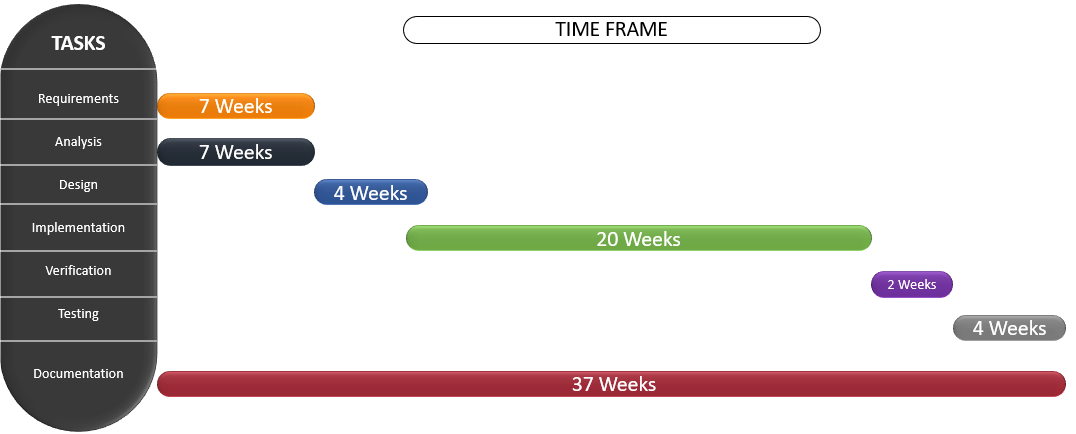
\includegraphics[scale=0.5]{gant.png}
	
	\newpage
	\chapter{Literature Review}
	\section{Introduction}
	Sentiment analysis is a field that allows interaction between human beings and computers using natural language. This field allows listening or paying attention to the customers feedback. It is being applied in different fields like politics, marketing and also learning. Sentiment analysis is the process of analysing opinions expressed in form of text computationally with normally a goal of obtaining the attitude of someone towards a certain topic / subject. This chapter describes sentiment analysis and the fields that are currently using it, effort that was directed towards using it and technologies that are currently being used to retrieve feedback from customers. Research unveiled that different algorithms have been in use for the use of sentiment analysis in different fields and these algorithms are also described in this chapter.

\section{Sentiment Analysis Definitions}
Different and multiple efforts were put in place with the aim of giving the best definition that brings out all the elements covered by sentiment analysis in a single line. The term itself has got different names that are used to means the same with it that suit best with the subject of application at a particular period of time. Authors are using the different names in accordance to the subject. It is sometimes called opinion mining \citep{pang2008opinion} and also polarity detection \citep{sharma2014polarity}.   \\
 \cite{inproceedings} defined opinion mining/sentiment analysis as a recent discipline at the crossroads of information retrieval and computational linguistics which is concerned not with the topic a document is about, but with the opinion it expresses. This definition is far much too broad and it put focus on document level sentiment analysis. Document level sentiment analysis is normally not appropriate as it take the whole document as a single entity. Therefore the definition is not specific enough to define sentiment/ opinion mining in library terms. \\
 
 \cite{priyasentiment} defined “Sentiment analysis is the process of analysing the affective text into positive ,negative or neutral emotions.” This definition misses out the techniques that are used that is Natural Language Processing, computational analysis and linguistic and textual analysis. Adding the techniques to the definition, a new definition which states that Sentiment analysis is a data mining type that looks for inclination from people’s opinions using natural language processing, text analysis and computational linguistics, which their use is to extract and analyse subject related information from different sources. This definition suits best sentiment analysis for a library system.\\
 In accordance to the field in which sentiment analysis is being applied that is Libraries, a specific definition of sentiment analysis can be derived. Sentiment analysis is the process of extracting library content viewers’ comments to see their feelings towards the content in the library (i.e. videos). \\
 
\section{Algorithms used in sentiment analysis}
Sentiment analysis uses different algorithms to perform the analysis and classification of the data points in the data sets. These algorithms are placed into categories. The categories include Machine learning approach, Lexicon based approach and hybrid approach. For machine learning, algorithms that are used to analyse and classify the sentiments include Naïve Bayes Classification Algorithm, K-Nearest Neighbour, Support Vector Machine Algorithm, Linear Regression, Decision making tree, random forest algorithms, Maximum entropy rule , Probability latent semantic and Latent Dirichlet Allocation \citep{jandail2014proposed}.\\
From the category of Lexicon based algorithm, there is Dictionary based approach, Novel Machine Learning Approach, Corpus based approach and Ensemble Approaches. Lexicon based approach uses sentiment dictionary that contains a number of opinion words and compare them with the data available and determine the polarity. Three strategies for constructing a lexicon of sentiment include methods based on corpus, manual construction, and methods based on dictionaries. Manual construction is a very difficult task and a very time-consuming task. Corpus-based methods have got relatively high accuracy when it is producing opinion words. Finally, in the dictionary based techniques, the idea is to collect a small and understandable set of opinion words in person / manually first with known orientations, and then to grow this set by searching in the WordNet dictionary for their synonyms and antonyms.\\
Finally, in the hybrid approach, that is the combination of the machine learning and lexicon based approaches has potential to improve sentiment classification performance. The main advantages of hybrid approaches are the lexicon/learning symbiosis, the detection and measurement of sentiment at the concept level and the lesser sensitivity to changes in topic domain. While the main limitation is that reviews are with a lot of noise (irrelevant words for the subject of the review) are often assigned a neutral score because the method fails to detect any sentiment.\\
Some researchers have been researching the implementation of machine learning technique since the beginning of this century to collect feelings from online reviews using this method, many researchers have viewed opinion mining as a question of text classifications \citep{jandail2014proposed}. This approach usually involves creating a model using statistical techniques such as Support Vector Machine (SVM) and Naïve Bayes (NB).\\
Choice of algorithms varies from application. Some situations require parametric machine learning algorithms and some situations requires non-parametric machine learning algorithms. Parametric machine learning algorithms these are algorithms that simplify the functions used to the known form and then use a number of assumptions. Non-parametric algorithms these are algorithms that do away with the use of string assumptions about the mapping functions form. Non-parametric algorithms are free to learn any functional form from the data used for training the model.\\
Discussing the mainly used classification algorithms
\subsection{Naïve Bayes Machine Classification Algorithms.}
This is one of the powerful machine learning classification algorithms. This is a method of classification based on the theorem of Bayes with strong (naive) assumptions of independence between features. A Naive Bayes Machine Learning classifier expects that the proximity of a specific feature (element) in a class isn’t connected to the proximity of some other elements.\\ 
This algorithm uses the likeliness of elements and as a result this brings a number of errors in the output that this classification algorithm outputs. For example, if an organic fruit that looks like an apple is entered in the system it will be classified as an apple. This applies the same to sentiments, understanding the difference between spam sentiments, conditional statements and positive and negative sentiments takes a very big amount of time.\\
Naïve Bayes doesn’t require a very large amount of data to train it. Very small datasets can be used to train it unlike SVM which requires a very large dataset.\\
Most we use it in textual classification operations like spam filtering. It attaches probability values to every word that belongs or that is associated with spams, in accordance to the topic or the company that is sending the email. The Naive Bayes is commonly used to classify texts into multiple classes and has recently been used for classification of sentiment analysis.\\
\subsection{Support Vector Machine Classification (SVM) Algorithms.}
Support Vector Machines is a type of supervised machine learning algorithm which provides classification and regression analysis data analysis. SVM is mostly used for classification while they can be used for regression.  Supervised learning algorithms these are algorithms that operate with labelled data. If a new data point is received the system compares the data point with the current data in the dataset that was used to train the model/ system, then conclusion is reached basing with the information used to train the system at first. SVM can solve linear and non-linear problems and it works well for a number of practical issues. SVM's idea is simple: the algorithm generates a line or hyperplane that divides the data into groups. A hyperplane in a Euclidean n-dimensional space is a flat, n-1-dimensional subset of the space dividing the space into two disconnected sections.\\
Support Vector Machine Algorithms are known to perform well in sentiments analysis classification \citep{abirami2017survey}. SVM investigates data, characterizes selection limits and uses the components performed in the input space for calculation \citep{harb2008web}. The important information is presented in arrangements of two vectors, where each vector is of size m. After, the machine tries to identify the boundary that’s separating the two classes that is far from any place in the training samples \citep{pang2002thumbs}. The separate characterizes the edge of grouping, increasing ambivalent choices by extending the rim. According to \cite{cherian2013providing} the SVM has been proven to perform more effectively than the Naïve Bayes classifier in various text classification problems.\\

\section{Advantages and Disadvantages of Sentiment Analysis}
Examining the metrics of the market one by one is not the best way to measure marketing performance. A more holistic approach, which requires combining different marketing metrics, will yield more detailed and insightful results. Sentiment analysis is one of the metrics providing the context needed to evaluate your marketing performance.\\
Having a lot of likes and comments under a video library posts might seem like a success. After all, people are interacting with the content, so the video library plan may seem like it’s working. To kill small bad comments while they haven’t spread any far there is need for sentiment analysis. The advantages of sentiment analysis are discussed below.\\

\textbf{Advantages}
\begin{enumerate}
\item \textbf{Sentiment analysis helps in developing a more insightful, data-based marketing strategy.}\\
Beating a strategy based of data is really impossible to archive. Sentiment analysis is one of the indicators that will advance marketing strategies since it has an effect on the online presence of many different aspects of the brand. Analysing the emotions around the brand helps understand the motivations behind the purchasing decisions of consumers and the motives behind their searches.\\ 

Sentiment analysis helps in getting data base on which it can bring the marketing strategy to the next level. In addition, sentiment analysis provides strategic information when it comes to assessing the rivals. Marketing strategy components should be present which help in distinguishing competitors. That's one of the benefits of analysing sentiments–it allows you to discover and leverage the unique parts of the videos offered.\\

The impact of marketing campaigns on the sentiments about the brand can be seen. Analysis of sentiments helps to identify audience groups that respond to content most positively. This will help deliver more personalized messages to the product's most targeted audience.\\

\item\textbf{ Understand your customers}\\
It's difficult to succeed in business without an audience full understanding. The more accurate the message is, the higher the response rate. Analysis of sentiments can be the secret weapon, not only in targeting the right demographics, but also in monitoring the overall tone of the talk. The application of sentiment analysis to the marketing portfolio would help to get the most out of the posted content. \\

\item \textbf{Take a look at brand perception}\\
Sentiment analysis helps and ensure that the messages shared are relevant and targets the right audience. One of the greatest advantages brand owners have is a strong understanding of a brand, by monitoring sentiments around the industry, they can see how people feel about some subjects and change the content accordingly. \\

\item \textbf{ Give extra boost to your customer service}\\
Once a crisis hits, there is need to take action so fast, before its escalation. Sentiment analysis helps to contain crisis around the brand, or even turn the tables around and use the crisis as an advantage. The key is acting fast and spotting negative comments early. This help to nip the critical situations in the bud.\\
 
\end{enumerate}
\textbf{Disadvantages}\\
While an analysis of sentiments is useful, there is no believing that it is a complete replacement for reading survey responses, as the comments themselves often contain useful nuances. Where sentiment analysis can further help by identifying which of these comments should be read, allowing, for example, to focus on the most negative comments.


\section{Existing related systems.}
\begin{enumerate}
	
	\item \textbf{YouTube}\\
	YouTube is a video sharing library. It’s much of a video sharing library. It allows users to create channels and upload videos in to their channels for people to see. It allows users to visit the channels like videos and comment and let the owner of the channels seeing all these comments. It caters for adult and children. This video library pays owners of the channel for the videos they upload. The channel owners are paid according to the number of view on their channels. This makes YouTube an employment video library. According to \citep{bartl2018youtube} the amount of YouTubers is over 13 Million and that is 13 million people working on YouTube.\\
	
	The problem that YouTube does not cater for is helping YouTubers to increase their market share. It does help the YouTubers to analyse the comments from the subscribers and viewers.
	
	\item \textbf{Facebook}\\
	Facebook is one of the sites that can be called social networking sites. It make it easier for people to connect and share information that include videos with family and friends over the line. By 2006 anyone over 13 year old was able to join Facebook as long he or she has a valid email address. As far as social networking topic is concerned Facebook is the largest social networking according to market share, it has got more than 1 billion users. \\
	Today people are making money through monetizing Facebook web pages. This makes Facebook another employment platform. There is money people are making out of YouTube so there is need to analyse the comments and help the owner of pages to see the extent to which their content is liked by their followers. If the followers are not satisfied then the system must help the page owners to see where they are missing it by highlighting negative and positive comments.
	
	\item \textbf{Vidyard}\\ 
	Vidyard actually offers a video library feature that are offered by the above discussed video libraries. These include having a central hub for videos, collaborating seamlessly, reducing storage and server costs, controlling video access for customers and easily making changes. All these makes up the benefits of Vidyard. The sentiment analysis part remains uncovered just like other video libraries.\\
	
\end{enumerate}

\section{Traditional ways of Capturing Voice of Customers.}
The traditional ways of capturing feedback from customers were so laborious and not effective at all than the currently being used methods. The effort that was needed to capture data from a single customer was so laborious. Examples of traditional methods that were used to capture the feedback include interviews, questionnaires, observation and focus groups. \\

Interviews is one of the methods that was used to allow customers to return feedback long in the days before introduction of a lot and present day found technology \citep{interview}. Interview is a process of gathering data when people stay in a room and they have a question and answer session. Where the interviewer ask questions and the interviewee answers the question. Interviews have got a weakness of directive questions. The interviewer asks what he wants to know and doesn’t allow a customer to say out what she things is wrong within an organisation. \\

Questionnaires is a sheet containing questionnaires that is send to person of interest. Normally it is passed to customers after service delivery and they answer the questions saying out their feedback. Then the questionnaire is analysed and conclusion is reached out of the questionnaire. Problem with this way of gathering feedback from customers is the questions it contained maybe directive in such a way that avoids the customers from clearly saying out a view with the fear of not answering the question. Questionnaires also does analyse the answers passed by responders alone \cite{mann1998not}\\

Observation is a feedback gathering technique that was being used in the past. Observation needs an observer that gathers the information from customers by observing them while they are in the place of interest. Then conclude from what the observer see from the movement of the customers and so on. The weakness with this technique is that customers can change their behaviour if they realise that they are under study. The other weakness may also come from the observer as the observer can be biased in the study and conclude in a way that satisfies him or herself.\\

Lastly focus groups was one the techniques that were used for gathering information from customers. Listening the voice of customers with focus groups calls for a meeting between the customers and a number of stakeholders of the firm or organisation. This technique has got a weakness of having very few stakeholders included \cite{Cc}.\\


\section{Existing technologies of retrieving feedback from customers}
	Libraries are using different ways of capturing sentiments from patrons. Some of these methods include suggestion boxes, emails, tawk.to,social media, and phone calls. All these methods are laborious and tedious to arrive at a conclusion using them. They need an extra hand or effort from top management that is of analysing the data till its making sense.\\
	
	Suggestion box is a device used to collect comments and feedback from customers about a service that they are being offered. Traditionally this was a box and with technology it changed to be electronic suggestion boxes. \cite{farnum2011can} did a research about how suggestion boxes are being used in Canadian academic libraries. The research was targeted to see how often do suggestion boxes used in libraries and how often do they use them. The research discovered that almost every academic library in Canada has got a suggestion box and they are still using the suggestion boxes. \cite{farnum2011can} suggestion boxes support four major aspects in service improvement. The aspects are accountability, trustworthy, decision making and anonymity. Suggestion boxes have got advantages of leaving comments anonymously. The identity of a customer is not exposed. Even if a patron drops a comment letter in the drop box while someone is looking it him or her no identity is exposed.  Suggestion boxes solves the problem of directed comments from patrons. Patrons leave their feedback without anyone questioning them what they want to ask like what focus groups do. Then this allows patrons to express their thoughts clearly. This way of gathering feedback from patrons has got disadvantages of eliciting dissatisfaction feedback and it will portray a negative image of library while there is a positive side of it too \citep{shenton2007library}. \\
	
	Phone calls is another tool that is being used to capture or listen to customer feedback \citep{dean2007impact}. Using this tool customer calls the library when there is a complaint or if there is a query which must want to be attended. This tool has got a number of disadvantages. It is really expensive for customer to call the library. This reduces the number of customers who calls the library, at the same time reduces the number of complaints that the library receives. Reduction of complaints end up portraying a wrong image about service delivery in the library. Management end up thinking that if there is no complains the service delivery is perfect.\\
	
	Customer support chat is one of the methods that is used to capture voice of customers. In this technique customers will interact with a person from the organisation who is responsible for communicating with the customers. The person is normally called the Customer Support Manger. A research was done by \citep{torstensson2017customer} with the aim of gathering facts to see if it was necessary to use a live customer support chat. Live customer support brings a number of advantages to both the organisation and also to customers. Live customer support motivates customers to launch complains as they are certain that they will get immediate response in real time (Pinto, 2013). It requires very little energy for a customer to submit a complaint or a suggestion. This helps the organisation to maintain its good will as it always responds to customers need. This method of listening the voice of customers is better than emails \citep{elmorshidy2013applying}.  By using live customer support chat, companies gain economic advantage to use of really expensive customer support call centre \citep{elmorshidy2013applying}. \cite{torstensson2017customer} concluded that a support chat can be used as a way of engaging with customers either new or old customers. However, the study didn’t look in a number of issues that are important to every organisation. It didn’t consider how economic it is to use live chat. Live chats need human beings to respond to customers. For very large organisations there is need for more Customer support managers for the organisations to respond to every customer in real time. This will increase cost to the organisation as it has to employee more workers.\\
	
	Use of social media platform such as WhastApp, Facebook, Twitter and Instagram is another method that is being used for getting feedback from patrons. Social media are websites and application that people uses to communicate, create and share information. Apart from its uses in organisation it has got its uses for entertainment purposes. WhastApp is used for chatting with friends and at the same time share documents, music, pictures and videos. Libraries have adopted these social media platform as a way of engaging daily with patrons. The main push is to follow the patrons in the place they are in. There are 7.7 billion number of people in the world and 3.7 billion are online \citep{ortiz2019rise}.  \cite{mabweazara2016assessing} research discovered that UK libraries use Facebook and Twitter more. Use of social media bring advantages of live communication between the patron and library staff. National University of Science and Technology (NUST) library and University of Western Cape (UWC) library are examples of libraries that uses social media to engage with patrons \citep{mabweazara2016assessing}. Social media has got its own disadvantages to use as a way of gathering patrons’ feedback.\\
	
	\textbf{Overview of Social Media Tools}\\
	
	\textbf{Facebook}\\
	Facebook is one of the top social media networks in terms of market share. It provides users with a platform to register and make friends of their choice by sending friend requests and accepting friends request. Friends are able to share ideas, photos, videos, comments, etc.\\
	
	\textbf{Twitter}\\ 
	Twitter is one of the world's most popular social media platforms with less market share than Facebook. It is an application for micro blogging that allows users to post short messages of up to 140 characters and less.\\
	
	\textbf{LinkedIn}\\
	LinkedIn is a social networking site mostly used by professionals from all disciplines to connect professionals of their interest from around the world. 2013 statistics report that LinkedIn has more than two hundred and fifty-nine million users around the world.\\
	
	\textbf{YouTube} \\
	YouTube is an incredibly well-known platform for video sharing that is used internationally for video sharing. YouTube is a repository for various video content styles including short video clips, TV clips, music videos, lectures on education, documentaries, films, games, etc. Individuals and educational institutions, media groups are increasingly using it to distribute their promotional material.\\
	
	\textbf{Flickr}\\
	Flickr is a website that is maintained by Yahoo! Inc. for photo sharing and video hosting, a free service that allows users to upload and share their desired digital images on the web with their groups or to the public. Flickr has an estimated 87 million registered members and over 3.5 million new images posted daily.\\
	
	\textbf{Pinterest} \\
	This is a pin board-style image-sharing website that allows users to create theme-based sets of photos such as activities, interests, and hobbies. Users can browse for images on other pin boards, "re-pin" images to their own pin boards and like pictures.\\
	
	\textbf{Orkut} \\
	Orkut is another social platform that has Facebook features. Users can connect with their friends through this website or create new friendships. They can comment on their friends ' shared posts, send certain messages, talk with them, and also upload pictures.\\
	
	\textbf{Tagged} \\
	Tagged is a platform for social exploration that allows its users to view other users ' profiles, play games, exchange tags and digital gifts etc. About 100 million users use this program, according to an estimate.\\
	
	\textbf{MySpace} \\
	MySpace is another popular social networking site that mainly has a social purpose that allows people to make buddies, chat online, and divide resources among themselves.\\
	
	\textbf{Google Plus} \\
	Google+ and Google Plus is owned and operated by Google Inc. as a social network site. It is known as the world's second-largest social networking site. According to a survey, this network contains 540 million monthly active users.\\
	
	\textbf{LiveJournal}\\
	LiveJournal is another social networking service that allows Internet users to maintain a blog, journal or diary, and is also the name of the free and open source server software running the LiveJournal website and online community. There are about 16 million publications on various topics such as politics, culture, fashion, literature and architecture, etc. on this social networking site. \\
	
  \textbf{Photo bucket }\\
	Photo bucket is a website that shares photos and saves footages. It is an online community dedicated to photos and videos preservation and sharing. Millions of users use this page to share with their loved ones their pictures and videos.\\
	
	\textbf{Picasa}\\
	Picasa is a platform for photo sharing that was used to organize and edit digital images.\\
	\textbf{Slide share} \\
	Slide share is a slide-hosting platform based on the internet. It provides users the ability to access documents in various file formats, such as PPT, PDF, Keynote and Open Document presentations, personal or publicly. Users can also rate, comment and share the content that has been uploaded. Slide share has been voted as one of the top ten educational and e-learning resources in the world.\\
	
	\textbf{Blog}s \\
	This application helps users to share data at one time with a number of people. Blogs are also helpful! And used to distribute circulars of offices and latest announcements of activities in universities on a very large scale.\\ 
	
	\textbf{RSS }\\
	RSS (Really Simple Syndication) is a web stream that includes full or correct text and information about changing metadata, new blog posts, news headlines, audio and videos, etc. The program helps users who want to update their favourite websites on time. Subscribing to a website's RSS service eliminates the user's need to manually check the website for new things. Alternatively, by updating the page and letting the user know about new updates, their app does this job.\\
	
	Social media has proved to be a reliable source of product marketing knowledge. A unique data source provides a quick means of customer feedback used to help a number of business areas. Social media can provide immediate feedback in minutes, thereby presenting a new challenge in customer-business communication. One can use social media to evaluate consumer reaction, along with relevant information, in the form of what they like (or don't like). This can benefit other areas of an enterprise, including product development, customer service or marketing.\\
	
	All of the above methods do engage with patrons in its own way. It has got disadvantages and its own advantages. In addition to the above disadvantages of each method there is a common disadvantage of not being able to analyse the sentiments / feedback that patrons pass. Thereby requiring third hand for the gathered sentiments to be useful, thus being laborious.
		
	\section{Existing Sentiment Analysis Systems}
	Sentiment analysis is a wide spreading concept that is penetrating almost every aspect of life. This concept has been applied in different subject areas that include politics, marketing, brand monitoring, customer support customer feedback and social media monitoring. Of late sentiment analysis applications focused on classifying film reviews or product reviews as positive or negative or distinguishing positive and negative sentences, but many recent applications include opinion mining in ways that require a more detailed analysis of the sentiment expressed in texts \cite{jandail2014proposed}. One such application is to find reviews of a product to see which area of the products rated good or bad by customers. Another task which involves a more detailed analysis of sentiments is to consider where political writers fall on the political spectrum, something that can be achieved only by searching for support or opposition to specific policies. A few other uses, such as allowing politicians who want a deeper understanding of how their voters view different issues, or forecasting stock prices based on opinions people have about the businesses and assets involved in the marketplace, can also benefit from organized representations of opinion. Sentiment analysis helps management to manage customer's feedback. There are a number of different sentiment analysis researches that were done in recent years. The aim depending from one research to another.\\
	
	
	Different authors tried to come up with researches on sentiment analysis application in hotels. \cite{kasper2012monitoring} undertook a research for a project which was done for Saarland hotel association. The project name was BESOHOT. The aim of the research project was to improve the information value. After the research the project was implemented pilot with the aim of improving the way Saarland value the Voice of Customers. \cite{grabner2012classification} also did a research about use of sentiment analysis in the hotels. The conclusion after the research was undertaken using lexical based approach to classify customer's feedback.\\
	
	\section{Proposed System}
	The system that is going to be developed is going to remove the common disadvantage of the current methods that are being used to capture sentiment/ feedback from patrons. The common disadvantage is waiting for third hand to make information useful. The proposed system is going to be developed using Python programming language and Django.
	
	\subsection{Python}
	Python is an interpreted, object oriented high level programming language that has semantic dynamic semantics. This programming language. This programming language is very easy to learn and easier to read code. This brings an advantage of easy to maintain code. It also have garbage collection features, that reduces the labour of the programmer during coding. The programmer doesn't have to worry about when to and when not to release no longer being used memory.
	
	Python is very popular open-source programming language. It offers the benefits of leaner code, shorter development cycles, compatibility with various platforms, backward compatibility, and streamlined security, administration and testing software development.
	
	\subsection{DJango}
	Django is a Python Web platform at the highest level that facilitates rapid development and clean, practical architecture. Created by seasoned developers, it takes care of much of the web development problem, so you can focus on writing your app without reinventing the wheel. It's open source and free.
	
	\section{Conclusion}		
	This chapter provided a brief overview of the systems that are currently being used in libraries to capture customer feedback and the definitions that are used to define sentiment analysis. The chapter was trying to shade out the advantages that sentiment analysis will bring to libraries if project undertaken.
	
	\chapter{Methodologies}
	\section{Introduction}
	Software development methodologies play a vital role in developing a system software. The basic purpose of these methodologies is to provide smooth software development according to the project requirements. Software development methodology ca be defined as a framework that is used to structure, plan, and control the process of developing an information system. This chapter look into the methodologies chosen for the research, development and implementation of this project.\\
	
	\section{Research Methodologies}
	Research is a careful consideration of the study using scientific methods for a particular concern or problem. According to the American Sociologist \citep{babbieadventures}, “Research is a systematic inquiry to describe, explain, predict, and control the observed phenomenon. Research involves inductive and deductive methods.” Methodologies are methods method used in a common area of study or operation. Combination of these two words forms research methodologies that is defined as the basic methods or techniques used to define, pick, process and analyse information about a library sentiment.\\
	 
	There are two basic categories of research methods in software development and they are qualitative and quantitative. They are applicable to numerical and non-numerical projects. Quantitative research methods support experiments and testing by measuring variables to verify or falsify theories and hypothesis must be evaluable and answerable. The method requires large datasets and use statistics to test the hypothesis and make the research system valid. The qualitative research method is concerned with understanding meanings, opinions and behaviours to reach tentative hypotheses and theories or develop computer systems, artefacts and inventions. The qualitative model mainly uses smaller datasets that are sufficient enough to reach reliable results, where the data collection continues until saturation is reached \citep{ghauri2010research}.\\
	
	Research methodologies define what activities constitutes research, how to proceed, how to measure and what constitutes the success of a project. There are generally five types of these methodologies which are Formal, Experimental, Build, Model and Process methodologies.\\
		
	\section{Formal Methodology}
	This type of methodology is used to prove facts about algorithms and systems. These formal methodologies are very popularly applied in theoretical computer science. In this project there is use of Support Vector Machine hence we can employ the use of the formal methodology to assess the algorithm. Formal methodologies will expose the complexity and strength of the SVM algorithm that will be applied in sentiment analysis of libraries. This helps determine the overall complexity of the operations in the system.\\
	
	\section{Build Methodology}
	Build methodology comprise much of building an artefact, either a software system or a physical artefact that will be used to demonstrate that it is possible to develop. In the situation or case of this project a build methodology that will be used must demonstrate that the software system can be built. To be considered a research, the construction that will be undertaken must demonstrate new artefacts features that haven’t been demonstrated in any other artefacts before. Whenever a research question leads to the building of a software system, there is a certain of good practices that should be considered which include designing the software, component reuse, choosing an adequate programming languages and testing the system all the time during the development phase.\\
	
	\section{Experimental Methodology}
	Experiment methodologies are used much more in the computer science field due to their ability to evaluate new solutions. Once there is a new solution there is need for it to be thoroughly evaluated to see the impacts of the new system and also if it’s feasible. The favouritism of a project is much based on its feasibility, that is the cost and the benefits it brings to the organisation as a whole.\\
	
	Experimental evaluation are divide into two phases normally. The phases are exploratory phase and the evaluation phase. The earlier mentioned phase –exploratory phase- the researcher undertakes some measures that will help in identifying the possible questions that may be asked about the software as a whole. The later phase that is the evaluation phase will attempt to answer these questions identified in the exploratory phases. For an experiment to be labelled as well designed it has to start with a well-structured list of questions that the experiment must answer. The main aim of experimental methodologies is to show the experiments that will occur with aim of extracting results from the real world implementations and they can be used to test a variety of theories.\\
	
	\section{Software development Methodology}
	During literature review, several types of software development methodologies identified which can be implemented in the sentiment analysis system to be developed. The literature has reviewed a number of methods that were used during different sentiment analysis researches and projects. To select the most suitable methodology, a proper analysis has to be done in the context of this project. Modern day methodologies are structured to minimise risk by developing software in short time boxes referred to as iterations which typically last one to four weeks. The iterations are sub-projects which include all the tasks necessary to release the increment of new functionality or for a different module of the system that exerts different actions to the final solution.\\
	
	There are factors that were considered for selecting the suitable methodologies. The major factors in the context of this project’s set up include the following:\\
	\begin{enumerate}
		\item \textbf{Complexity of the system.}\\
		The complexity of the project doesn’t allow or doesn’t work very well with traditional methodologies. Traditional methodologies are good at managing management system where there is really need for requirements elicitation. Traditional methods can’t be used in sentiment analysis (machine learning).\\
		
		\item \textbf{System Objectives.}\\
		The objectives of the project are not yet certainly specified, there is room of changing the objectives of the system in due course. The project goals and objectives were specified with a single human being (the student) that leaves the objectives at risk of being changed as time moves on after analysis from the project supervisor.\\
		
		\item \textbf{The availability of expertise.}\\
		The only expertise at hand are two humans being a naïve programmer (Student) and management (supervisor). The methodology that will be used must take note of the above specifications.\\
		
		iv.	\textbf{Cost involved in the project.}\\
		The project has no budget hence we would require the methodology that is not costly to implement.\\
		
		\item \textbf{Risks associated with the project.}\\
		Project failure will result in the student obtaining a poor grade or even failing but apart from that no other risks are associated with the project. A methodology that reduces the extent of risks can be used so that the student can get a good grade for the project.\\
		
		\item \textbf{The availability of resources.}\\
		In the student’s hands there is a single laptop and a cell phone that will be the device to use during project development hence methodologies that employ the use of other tools are neglected.\\
	\end{enumerate}
	\subsection{CRSIP DM}
	\textbf{	CRISP DM }stands for Cross-Industry Standard Process for Data Mining. CRISP DM is a methodology that is applied much in data mining but it is considered to be a standard methodology applied to the extraction of knowledge from big data sets \citep{sharda2016business}. Sentiment analysis works with datasets for training of systems either training the system using supervised learning algorithms or unsupervised learning algorithm. Due to the its ability to work with datasets, CRISP-DM was used by \cite{nave2018decision}.\\
	
	CRISP-DM has got six steps that are business understanding, data understanding, data preparation, modelling, evaluation and deployment (Chapmanet al., 2000).\\
	
	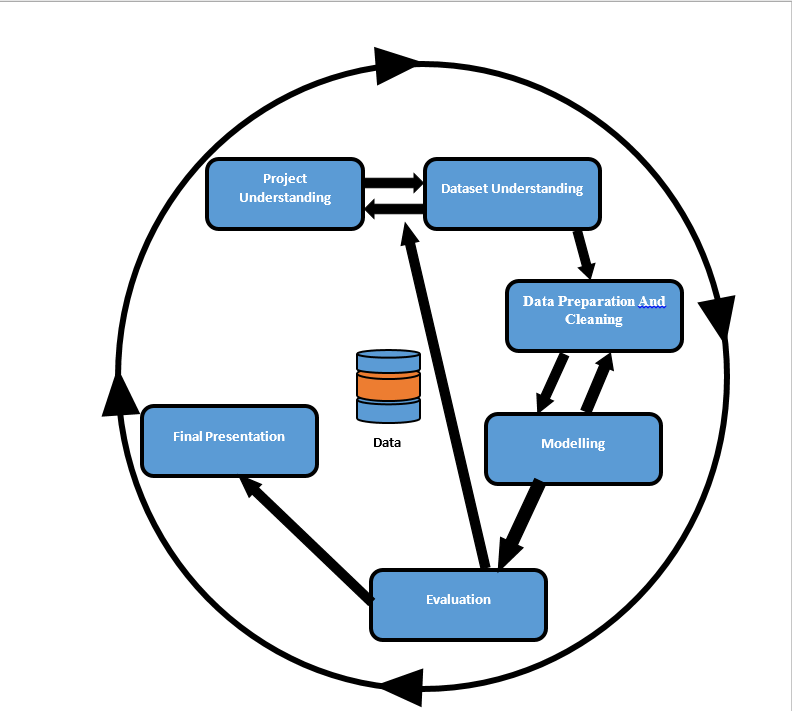
\includegraphics[scale=0.5]{crisp.png}
	
	\begin{enumerate}
		\item \textbf{Project Understanding (Understanding project goal)}\\
		The stages start with understanding the project goals. There is need to understand what the project is exactly about and knowing the expected outcome of the project. After understanding the objectives of the project then the knowledge in transferred into machine learning objectives.\\
		
		Situation assessment is also done at this stage to see the risk that may arise and providing contingency plan to the risks. Assumptions that will be used in the project are gathered and some constraints of project success are noted down.\\
		
		Development of a project plan is done at this stage this will lay the root that will be followed as the project proceed.\\
		
		\item \textbf{Data Understanding}\\
		This phases starts with data collection that is searching for possible datasets from reliable datasets. Analysis of the necessary procedures that are needed to have the datasets. Identification of data quality problems that will help to see if the data will help meet the project objectives or not basing on the field in which sentiment analysis is been applied.\\
		
		After this process initial data collection report, data description report, data exploration report and data quality reports are expected to be produced.\\
		
		\item \textbf{Data Preparation}\\
		After the initial data was collected there in need now to produce a perfect data set that will be used in sentient analysis. The first step is to describe the dataset this gives a view to project members what the data set collected about and what it is about to be used. After description the data is selected and the cleaned to remove unnecessary data in the dataset. Then finally the data is constructed, integrated and formatted.\\
		
		At the end of the phase there is data cleaning report, and formatted data.\\
		
		\item \textbf{Modelling}\\
		
		In this phase various techniques are selected and then the appropriate one is selected. The modelling assumptions are stated here in a try to perfect the environment and to create a ground that will reduce criticism of the model. The model test plan is set aside and the model is built. After the building process is done assessment is done to measure the success of the model.\\
		
		\item \textbf{Evaluation}\\
		The model or models produced are thoroughly evaluate to see if they went through the correctly stated procedures and see if all the assumptions stated during modelling were properly followed.\\
		
		\item \textbf{Deployment}\\
		The model is now functioning. The model is then presented to the intended guest or customers. The customers are taught how the model works.\\
		
		After that the project is placed under monitoring to see how it will continue functioning. \\
		
	\end{enumerate}
		
	\subsection{KDD}
	The \textbf{KDD} process, as presented in \citep{fayyad1996kdd} is the process of using DM methods to extract what is deemed knowledge according to the specification of measures and thresholds, using a database along with any required pre-processing, sub sampling, and transformation of the database. There are considered five stages, presented below.\\
	
	\begin{enumerate}
		\item \textbf{Selection }\\
		This stage consists on creating a target data set, or focusing on a subset of variables or data samples, on which discovery is to be performed.\\
		
		\item \textbf{Pre-processing }\\
		This stage consists on the target data cleaning and pre-processing in order to obtain consistent data.\\
		
		\item \textbf{Transformation }\\
		This stage consists on the transformation of the data using dimensionality reduction or transformation methods.\\
		
		\item \textbf{Data Mining}\\
		This stage consists on the searching for patterns of interest in a particular representational form, depending on the data mining objective (usually, prediction).\\
		
		\item \textbf{Interpretation/Evaluation} \\
		This stage consists on the interpretation and evaluation of the mined patterns.\\
		
	\end{enumerate}
	\subsection{SEMMA}
	SEMMA methodology is a methodology that stands for Simple, Explore, Modify Model and Assess. This methodology is more of a data mining methodology. Its help it’s much in data mining applications development. It can be said it’s a logical organisation tool set by SAS Enterprise Miner with the intentions of undertaking core data mining tasks. This methodology was developed with much focus into data mining application (Enterprise Miner) and other methodologies (such as CRISP DM) where developed to suit a wide range of data mining applications. SEMMA has got five stages that also makes up the abbreviation. The stages are Simple, Modify, Model and Assess.\\
	
	\textbf{SEMMA stages.}\\
	
	\begin{enumerate}
		\item \textbf{Sample.}\\
		The first phase of the SEMMA methodology is Sample. This phase is all about data sampling. This include processes like selecting the data set for modelling. The selection of a data set is a crucial process that must be treated with higher priority.  The dataset that will be selected must be enough or big to provide sufficient information needed and small to be usable efficiently. Data partition functionality is dealt with at this phase of the SEMMA methodology.\\
		
		\item \textbf{Explore.}\\
		This phase focuses much on data understanding. By understanding data there is need to discover the unanticipated and anticipated relationships between the variables and their abnormalities. To understand this there is really need for data visualization.\\
		
		\item \textbf{Modify.}\\
		The selection, creation and transformation of variables in preparation for data modelling are done at this stage.\\
		
		\item \textbf{Model.}\\
		The phase where there is vast application of various different modelling techniques. The techniques are applied on the variables prepared in the modify phase. All this is done so as to create models that provide the desired software outcome.\\
		
		\item \textbf{Assess. }\\
		The last phase is of the SEMMA is Assess. The results of the process will be finally out and then there is need to assess them and see if they have met the objective.\\
	\end{enumerate}
The Sample and Explore stages of SEMMA they have got some sort of similarity with Data Understanding phase of CRISP-DM. Modify can be translated to the Data Preparation phase. Model likewise is the Modelling phase. Assess is parallel to the Evaluation phase of CRISP-DM. All these models are expected to go in a cyclical way rather that linearly.\\
	
	
	\section{Chosen development Methodology}
	For research purposes the Build methodology was adapted. The reason behind the selection of this methodology is much based on its ability to cater and support system design, selection of programming languages which makes it flexible for code reuse in the event of upgrading the system itself. The other feature of Build methodology that called for its selection is its ability and mechanism of continually testing of system during development other than testing only after the project is completed. The system that will be built need continues testing because of the little know how of the programmer. The type of dataset that will be used need some thorough cleaning and to see if the dataset is clean and meeting the required threshold there is need for continues testing.\\
	
	For software development methodology the CRSIP DM methodology is the one that is going to be used. The selection of this methodology is much based on the steps of the methodology that are followed. The steps of the methodology suits the type of project that is being undertaken with little changing efforts. Other that other methodologies that are much in Data Science projects.\\
	
	\section{Development Tools}
	The project will be based much on python programming language for the back end. The front end will be based on python and some Gibrish. The text editor that will be of use is Visual Studio Code text editor. Django will be the frame work of choice for the full development of the system.\\
	
	\subsection{Python}
	Python is an interpreted, object oriented high level programming language that has semantic dynamic semantics. This programming language. This programming language is very easy to learn and easier to read code. This brings an advantage of easy to maintain code. It also has garbage collection features that reduces the labour of the programmer during coding. The programmer doesn't have to worry about when to and when not to release no longer being used memory.\\
	
	\subsection{Visual Studio Code}
	Visual Studio Code (VS Code) this is a source code editor or text editor developed combinatorial by macOS and Windows. It supports code debugging and syntax highlighting. It also has embedded Git control and GitHub. Moreover it has intelligent code completion, refactoring of code and snippets. It is customizable, enabling users to set the themes, keyboard shortcuts, preferences, and install additional feature extensions. All the functionalities and specialities of VS Code make it suit for these project. \\
	
	\subsection{Django}
	Django is a Python Web platform at the highest level that facilitates rapid development and clean, practical architecture. Created by seasoned developers, it takes care of much of the web development problem, so you can focus on writing your app without reinventing the wheel. It's open source and free.\\
		
	\section{Conclusion}
	The success of every project is much of in the hands of the methodology that is chosen. The methodology lays a way that the project team (no matter the size) must follow. Meeting of deadlines, coordination between team members and meeting objectives they all rely on the methodology of choice. This chapter has culminated in the choice of the methodologies that suits this project that is CRISP DM and Build Methodology. Methodologies give a guide to how the project as a whole is going to be undertaken. This methodology determines the success of the proposed system. The methodology adopted impacts directly the cost, the quality and time that will be taken to develop the project as a whole, this implies a direct influence on the success of the solution. A strong correlation is required between the research and development methodology as both are tools used to successfully create a solution.\\
	
	\chapter{System Analysis and Design}
	\section{Introduction}
	System analysis and design focuses on the intrinsic and deep analysis of sentiment analysis, the detailed flow of entities, architecture and the design of the system. This is a comprehensive architectural overview of the system, using different analytic tools to depict different parties of the system. Sentiment analysis activities were executed in accordance to the chosen methodology (CRISP DM). Systems analysis and design deals with planning, analysis, design and implementation of the build system. Along the phases the developer deals with the planning of the information system through understanding and specifying in detail what the system should do and how the components of the system should be implemented and work together. Logically the preliminary stage of software development is to establish precisely and accurately what the users of the system want. The dominant part of this stage is communication between the users and the software developer. When the engineers is dealing with requirements, he/she is normally referred to as a systems analyst or, simply, “analyst”.\\
	
	\section{System Analysis.}
	System analysis focuses on the process of collecting factual data understanding the process involved identification of problems in the data and preparing the data for the model.\\
	
		\subsection{Data Understanding}
	This project is based on the CRISP DM system development methodology. The six stages of the CRISP DM contains Data Understanding as the second stage of the development cycle. After the first stage of the cycle that called for understanding the project and its goals, the second stage guided in finding the correct dataset that will help to build the sentiment analysis model using Support vector machine - the model of choice.\\
	
	The data that is suitable for the system is textual data. Textual data contains different words of which some contains sentiment value and others don’t. The dataset gathered was from Kaggle that was gathered from YouTube video comments.\\
	
	The dataset was about 300 MB in size. The format of the dataset was \textit{.csv} and it had 1048576 rows and 6 columns. The dataset was a labelled dataset and one of the columns contained the sentiment value of every sentiment. The others column contained the sentiments. The feature of the dataset being labelled made this dataset suitable for use in this project as it removed the need for labelling the dataset. It didn’t call for reading each and every sentiment and understanding it before loading the dataset in the model.\\
	
	The dataset wasn't clean. It contained all types of symbols and short words that people use when communicating on daily basis. It also contained emoticons that people use to express their emotions. So there was need to deal with the emoticons too to make them valuable in this project.\\
	
	Since the sentiment analysis is for video libraries, dataset from YouTube comments was really suitable as YouTube is also a video library. YouTube also contains videos from different subjects of life that makes the dataset suitable for generalised video libraries. The sentiment analysis isn't for a specific chapter of life, but for general videos.\\
	
		\subsection{Exploring and Processing  Dataset(Data preparation)}
	The third stage of the CRISP DM is data preparation. Preparation of dataset is exploring and processing the dataset so that it fits perfectly well and also produces reliable model results. In trying to do so a number of processes are done that where much of data cleaning processes. All the data preparation stages were seen necessary after understanding the data structure in stage two of CRISP DM.\\
	
	For a sentiment analysis to work well some data features must be removed. This will save time taken by the system analysing data since some features that are used when people are communicating contains no sentimental value at all. In trying to pave or remove features without sentimental value a number of processes were done to the dataset as the steps for cleaning it.\\
	
	\begin{enumerate}
		\item Column deletion.\\
		The first data cleaning stage that was done was to remove some columns from the dataset. The dataset contained 6 columns of which the columns of value to the project where only two, the sentiment value column and the sentiment column. Other 4 columns where the date and time column, user id column, user name column and the other column which was written ‘NOQUERY’ throughout to the 1048576th column. The column removal was necessary as a way to reduce the dataset size.\\
		
		\item Lowercase.\\
		The dataset contained mixed text sizes that is capital letters and small letters. While the sentiment value between "LOVE" and "love" are the same. So to keep the dataset in a uniform format and to make sure a word in caps and in small caps are treated the same there was need to change the data to lowercase. To make this work \textit{lower()} function from python was used as shown below.\\
		
			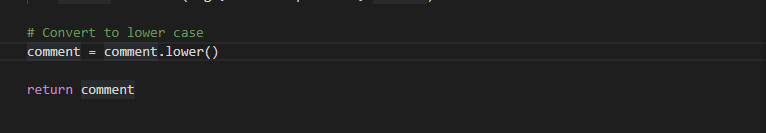
\includegraphics[scale=0.5]{lowercase.PNG}
		
		\item Removing Punctuation.\\
		Removal of punctuation symbols from the dataset was also necessary as the dataset contained a number of punctuation symbols. Punctuation doesn't add any extra information to the sentiment value. Removal of punctuation symbols reduce/ scales down dataset size and also improves computation efficiency of the model. For this feature \textit{regex} and \textit{replace} python function were used.\\
		
		\item Removing Stop words\\
		Removal of words that carries no sentimental value was a necessary step in this project. So stop words were also removed. Stop words are very common words that carry no meaning or less meaning compared to other keywords. If we remove the words that are less commonly used, we can focus on the important keywords instead. Making the model know best the well and commonly used words.\\
		
		\item Tokenizing data.\\
		Tokenising is splitting text into minimal meaningful units. There is a sentence tokeniser and word tokeniser. The one that was used in this project was a word tokeniser. The reason for using the word tokeniser was to ensure the model uses perfectly tokenized words, this improves model accuracy. Though this valued accuracy over time and CPU overuse. For this task \textit{trim()} method from \textbf{nltk} package was used. The reason was its simplicity approach to tokenizing data.\\
		
		\item Stemming.\\
		Stemming was used so as to try to extract root words from the words that were contained in the dataset. Words like "like", "likes" and "liked" were being stemmed into "like". Stem function from \textbf{nltk} library was used for this feature.\\
		
		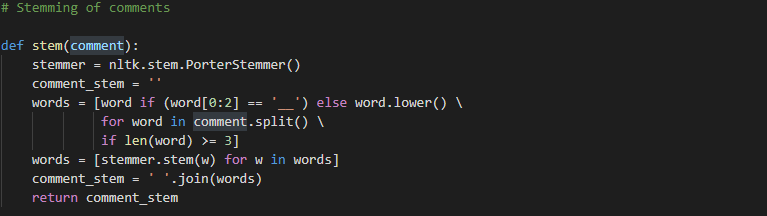
\includegraphics[scale=0.5]{stemming.PNG}
		
		\item Emoticons.\\
		The dataset contained sentimental value and the sentiment value need to be extracted as well. For this feature a small dictionary was created for emoticons that are positive and negative. Then the sentiments in the dataset were being compared with the small created dictionary as shown below.\\
		
		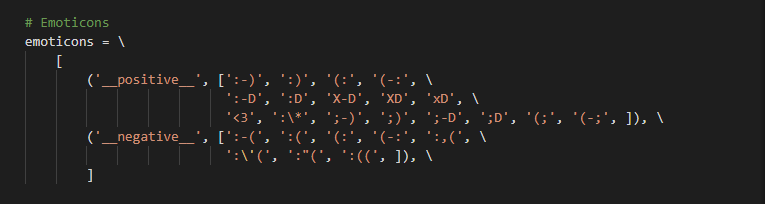
\includegraphics[scale=0.5]{emoticons.PNG}
		
	\end{enumerate}
	
	
	\section{Feature Engineering.}
	Feature Engineering is the procedure of converting raw text data into machine understandable format (numbers). For this project there was need to convert the dataset into a format that the model will understand before passing the data into the model. Different feature extraction methods can be used that include TF-IDF, One Hot Encoding, N-grams, Count Vectorizer and Hash Vectorize.\\
	
	Each of the above methods have got an area in which they suit best and for the sentiment analysis project TF-IDF (Term Frequency- Inverse Document Frequency). The suitability of the method is measured based on the type of the data and the structure of the data. The feature that need to be engineered so as to end up with highly accurate results in the model also helps in considering the method.\\
	
	The problem that was in the dataset was the repetitive occurrence of the same words. For example the repetition of the word "love" throughout the dataset. This was causing a bias in the outcome of the model since a repetitive appearance of a word achieve higher importance in other methods that was first tried that are Count Vectorize and Co-occurrence.  TF-IDF deals with this problem to avoid repetitions of words overpowering other words with sentiment value within a statement.\\
	
	TF-IDF is a combination of TF and IDF. Term Frequency is the ratio of the count of a word present in a sentence to the length of the sentence. TF just basically captures the importance of the word with respect to the length of the document. This implies that a word with frequency of three within a sentence with length ten is not the same as when the word length of the sentence is 100 words. It must get more importance.\\
	
	Inverse Document Frequency (IDF), of each word is the log of length of the total number of rows to the number of rows in a particular document in which that word is present. IDF measures the rareness of a term. That is a word is appearing in almost all documents, then that word is of no use to us since it is not helping to classify or in information retrieval. IDF will nullify this problem.\\
	
	\section{System Design}
	System design focuses on designing the architecture of the interfaces, the modules and the data for the system to satisfy the required requirements of the product/ system (Hull et al, (2017). This is now the application of all the theories about the system into development of the product. The aim of the design phase is on how to accomplish the system objectives.
	\\
	
	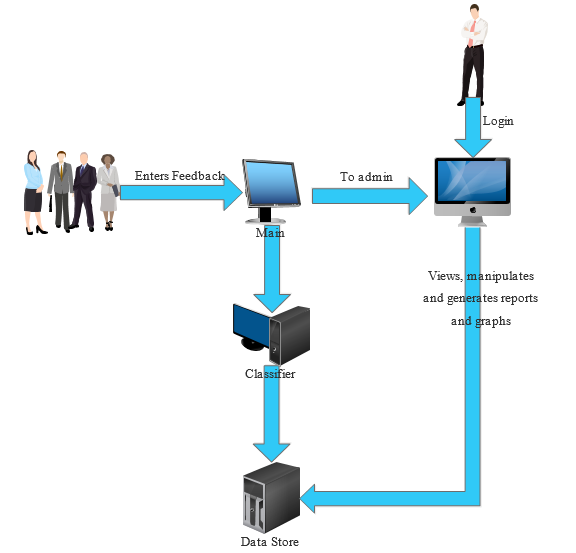
\includegraphics[scale=0.5]{aka.png}
	
	\section{Database Design}
	By database design we will be trying to produce a detailed model of the database. This include all the logical and designing choices and the physical storage parameters needed for generating a designing a data definition language. The data definition language is the one that can be used to generate or create a database.\\
	
	\subsection{Entity Relationship Diagram}
	An entity-relationship diagram (ERD) is a data modelling technique that graphically illustrates an information system's entities and the relationships between those entities. The elements of an ERD are entities, relationships and attributes. The Entity relationship diagram below shows the entities that are modelled to the system database and the association between the entities.\\
	
	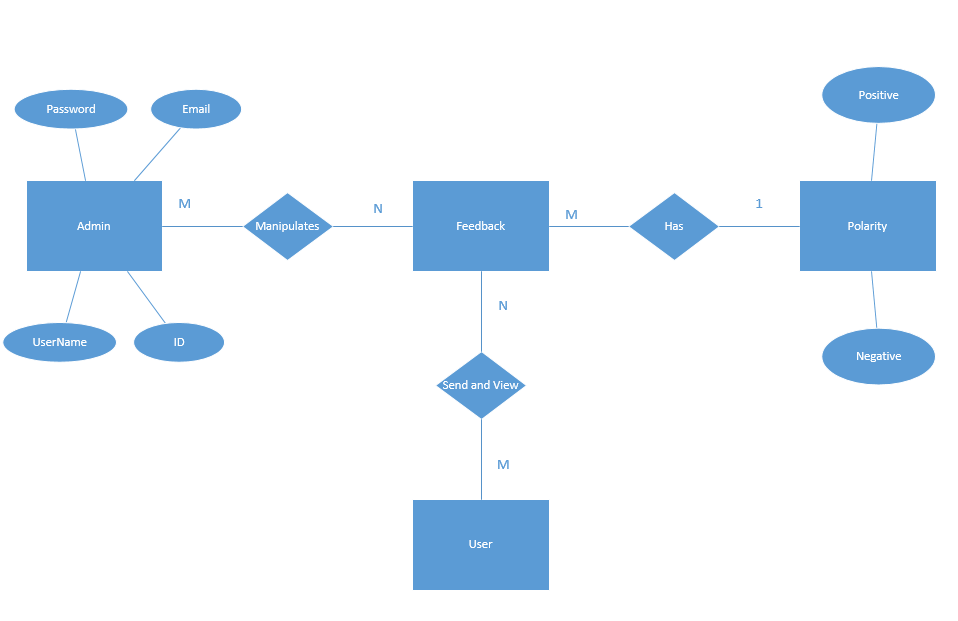
\includegraphics[scale=0.5]{erd.PNG}
	
		
	\section{System Modelling}
System modelling helps to visuals how the system work and interacts with external systems and objects. The modelling tries to visualise the requirements of external entities separately from the internal designs. Once there is a visualization of how external objects and internal objects will interact this aid in the development of the system as a whole. The easier it is to develop the sentiment analysis system the faster objectives are met. In other words system modelling marks the start of the implementation and testing phase of the software development methodology. According to the methodology chosen (CRISP DM) the stage of modelling helps to see if the project was clearly understood. If well understood then proceed to evaluation stage, on condition that the modelling stage is completely done. If the modelling stage is failing to come out well then a push back to understanding the project objectives is required.\\ 
The models will be used as a basis for system tests, making a clear relationship between the tests and the objectives and when the objectives change, this relationship is used to update the test.\\ 
	
	\subsection{Use Case Diagram}
	System have got behaviours. The behaviour of the system need to be visualise. One of the tools that visualise the behaviour of the system best is use case diagrams. Use case diagrams is an object oriented model construct. 
	Interactions between the user and the system are described through a prototypical course of actions along with a possible set of alternative courses of action (Grechanik et al, 2007). The use case diagram of the video sentiment analysis system is shown in figure below.\\
	
		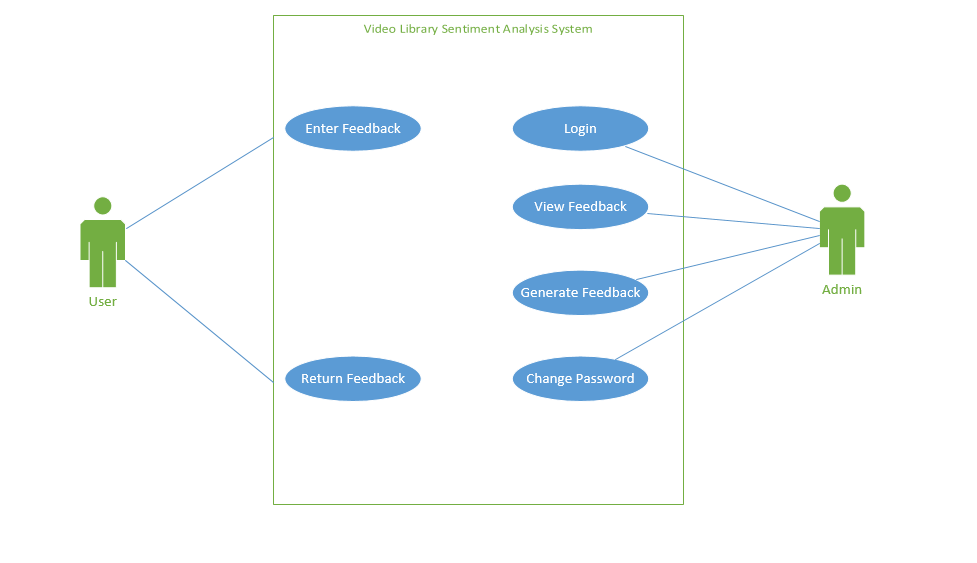
\includegraphics[scale=0.5]{usecase.PNG}
	
	\subsection{Activity Diagram}
Events in a system need also to be clarified. To show them clearly an activity diagram can be used. Unlike other diagrams this helps to visualise activities. It gives the overall view of the system showing all the possible results of an event occurring and how they tangled. Below is an activity diagram of the sentiment analysis as whole for a standard sentiment analysis.\\

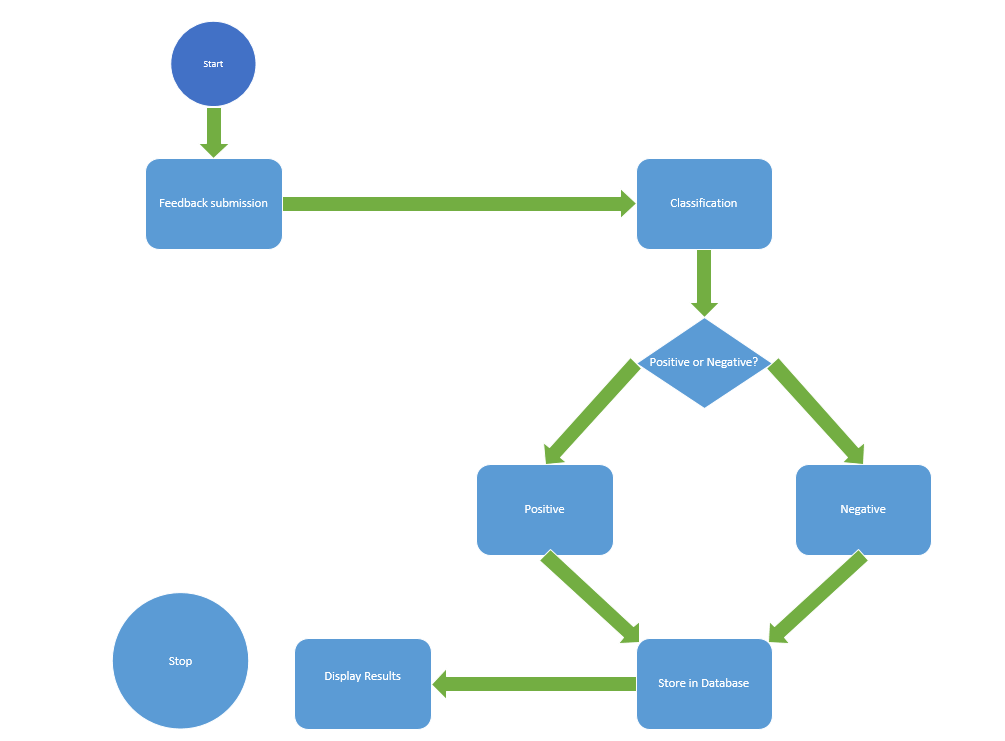
\includegraphics[scale=0.5]{activity.PNG}

\subsection{Sequence Diagrams}

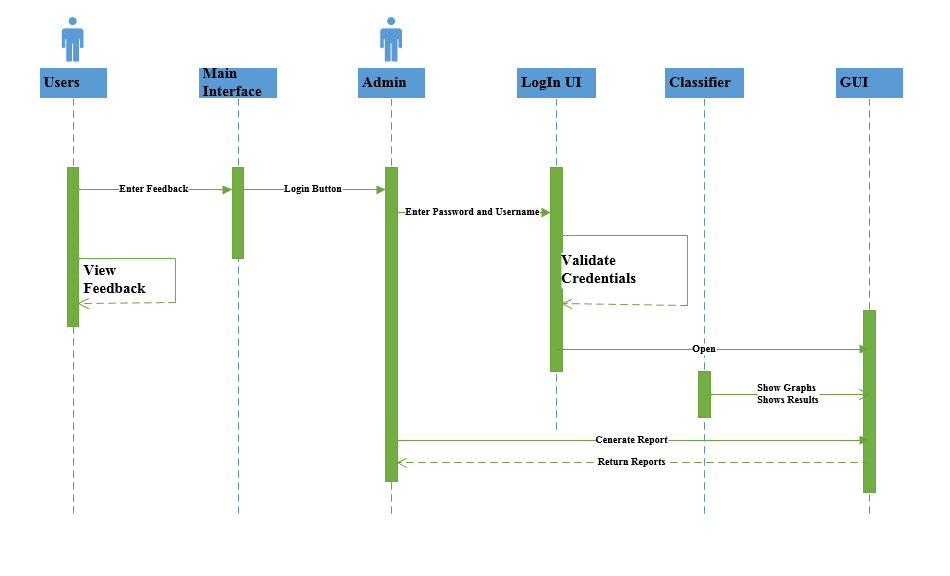
\includegraphics[scale=0.5]{sq.PNG}
	
	\section{Conclusion}
	
	This chapter discussed the system requirements elicitation process which is the most important stage in the software development process as it ensures that a system being developed fully satisfies the client needs. With the help of UML diagrams were also incorporated to define and discuss the analysis and design concepts of the system using use-cases, class diagrams, sequence diagrams and activity diagrams which convey the structure and functionality of objects in a way that can be better understood by the developers. The analysis and the design phases provided the foundation for the implementation of the system.\\
	
	\chapter{Implementation and Testing}
	\section{Introduction}
	After the stages of the CRISP DM that deals with data preparation, making it ready for use in the model, comes the Implementation and testing stage. This stages in the CRISP DM are called the modelling and evaluation stages. This marked the start of the development of the model. Different models were built with plan to see which one works well and then they went through evaluation as a way of comparing. 
	\section{Development Environment}
	Django development was set for the development of this project. From all available wide range of Development environments Django fell to suitable for this project due to a number of advantages. These advantages affect the probably end user of the model and mainly the programmer.\\
	
	The main reason behind the choice of Django was its capabilities to combine HTML codes with Python codes with easy. This advantage was mainly for the programmer since the programmer was much used to PHP programming. The imagination of how HTML is combined with PHP was the guide in development of this project. With that in hand Django made it easy through its internal instructions from pre-prepared files.\\
	
	Django also has the build in codes that it comes with that are of much help when starting Python development for the first time. The files are a guide/ tutor on their own to anyone who is starting Django for the first time.\\
	
	DJANGO has a private security key that insures security on the developed system. The code makes hacking of DJANGO programmed system harder to deal with (not impossible) with if you don’t know the password. The security key must be kept private to make the system secure after production.\\
	
	\subsection{Programming Languages}
	Python programming language was used for the programming of the system. Python is the code that was in charge of the whole model and the testing of the model. The reason for the choice was it capability to deal with relatively complex situations with easy. Python is also one of the programming languages that are easy to understand in terms of syntax as its syntax isn’t complicated that much.\\
	
	In building the user interfaces HTML codes were used under DJANGO control as it was the development environment. HTML was chose as it produces high quality user interfaces.\\
	
	The final product was then derived under DJANGO conditions with installation of some DJANGO plugins such as bootstrap and rest framework.\\
	
	\subsection{The Graphical User Interface}
	The GUI was developed using the HTML language in DJANGO and the development was guided by the 10 heuristics for interface design defined by Jakob Nielsen. Cognitive dimensions of notations also came into play and influenced the design of the graphical user interface. There are a number of colors on the GUI. There is a notable different in colors on the side that general user see and what the system Admins can see. This was done so as to allow clear recognition when someone entered the Admin section.\\
	The general view of everyone contains yellow as the main color and some white text on yellow bands and black where there is white as a back color. The general view home page is shown below.\\
	
	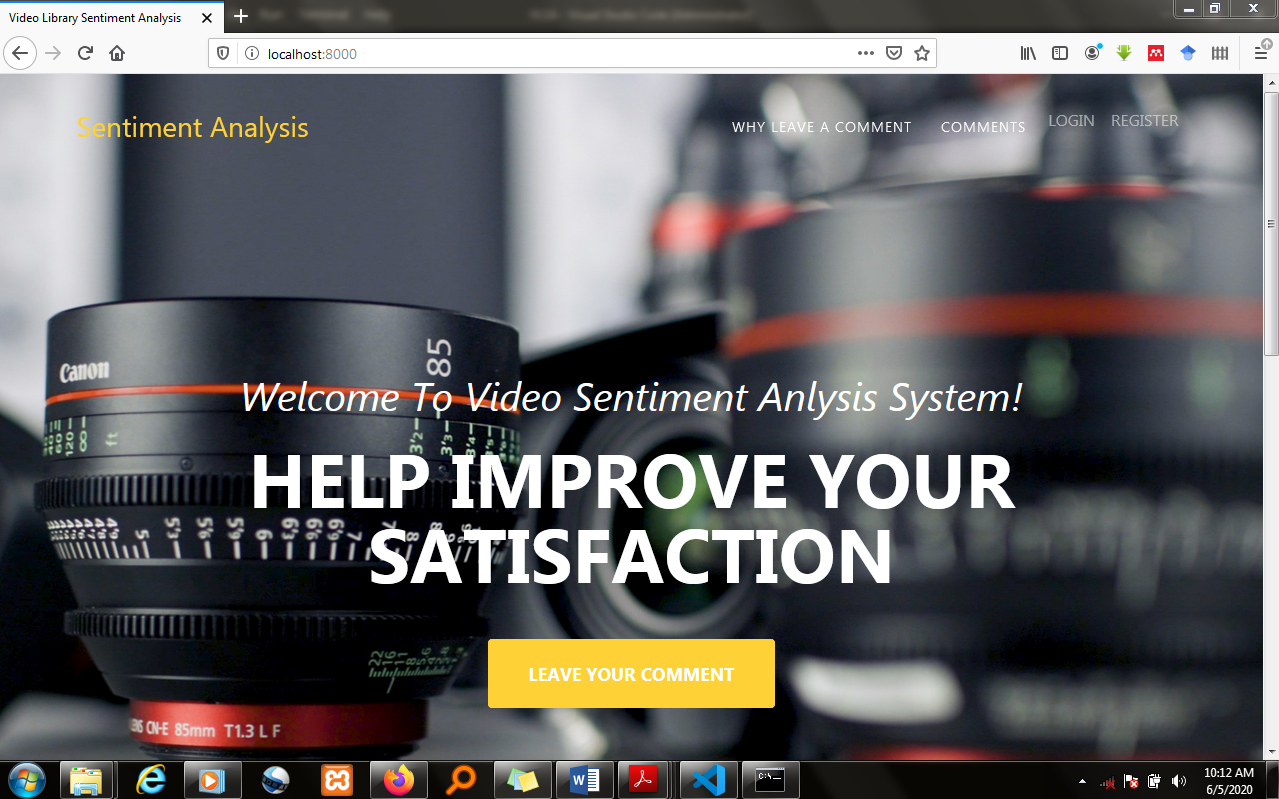
\includegraphics[scale=0.5]{home.PNG}
	
	The below view is the view of the admin’s panel with different colors from the general view. This is where all the logical activities of the system are done by system admins.
	
	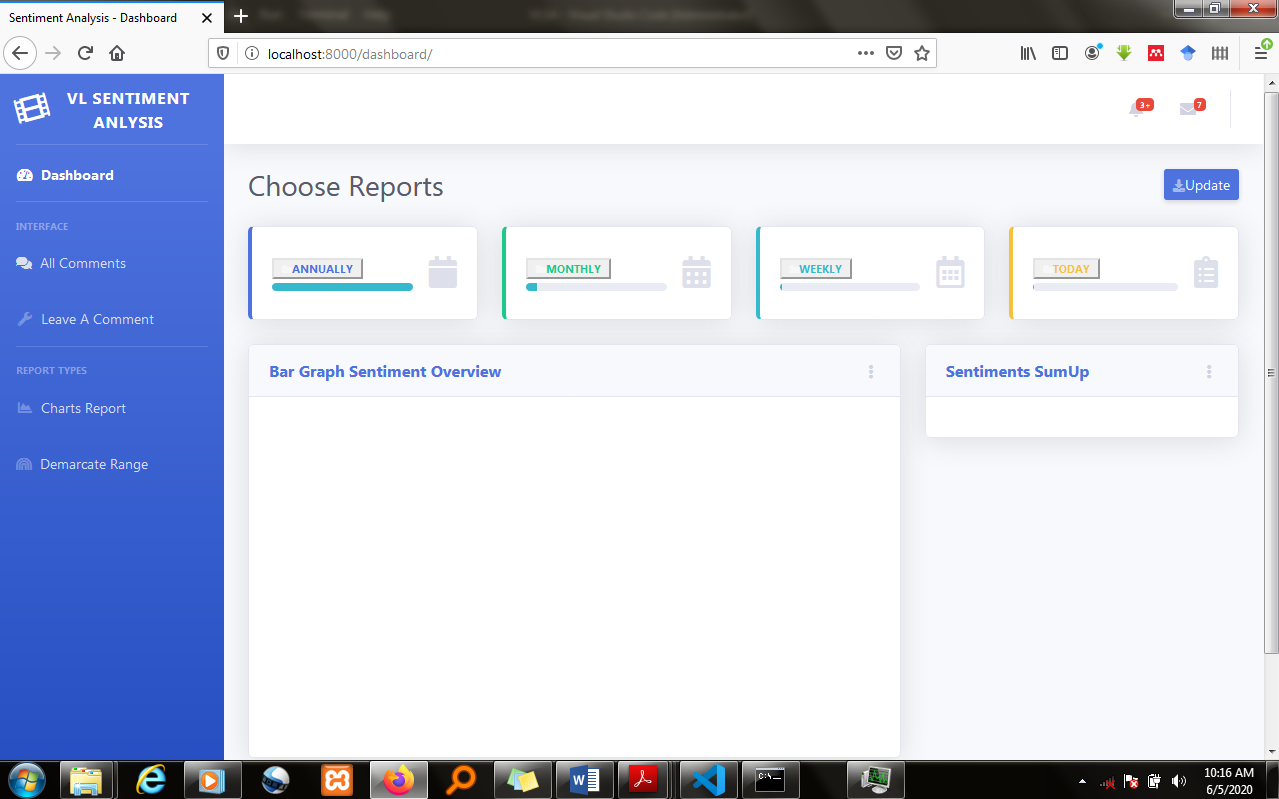
\includegraphics[scale=0.5]{admin.PNG}
	
	
	\section{Testing}
	This stage of the CRISP DM (evaluation) software development methodology was done so as to see if the system met the objectives. Testing is an iterative process where each logical unit of code is tested. The process is done of different entities if the objective isn’t met then we pull back to understanding the objective and plan again how to tackle it. The testing of a conventional software system involves some of the following phases.\\
	
	These are:\\
	
	\begin{itemize}
		\item Unit Testing.
		\item Integration Testing.
		\item System Testing.
	\end{itemize}
	
	\subsection{Unit testing}
	A software module can be created by building up of many small parts into a single module. This small part is called as a unit. A unit is a piece of code that will perform a specific task. At the end of this testing all units will be tested so that we can get the correct result. By using unit testing we can easily identify the errors.\\
	
	In this project a number of units where tested that include testing the model during development and also the user interfaces. While tackling this testing a number problems were met that were much of the model’s errors. The model was continually tested and changes to the code being done until the accuracy reached 88\% as shown below. Changes that were done on the model that improved the accuracy was the change of the feature engineering tool from Hash Vectorizer to TF-IDF. \\
	
	\subsection{Integration testing}
	Combining all programs into a single application and testing its correctness is called as Integration testing. Even all programs work correctly they may give a false result when they work together. Integration is very important to get the completed result.\\
	
	Integration testing was so troublesome, this was done to integrate the user interfaces and the model. The integration was aided by Django. A number of problems were met. These included a number of errors that are listed in the error log that I personal created for myself.\\
	
	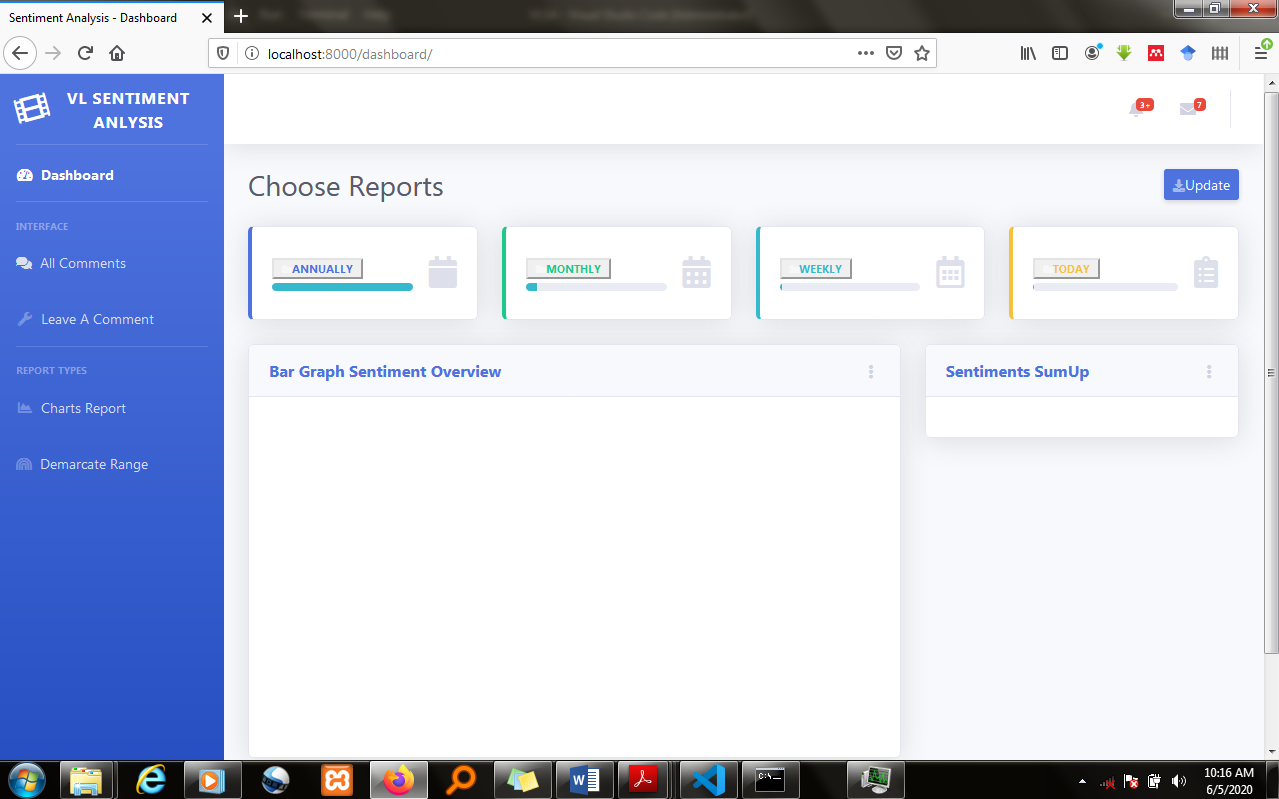
\includegraphics[scale=0.5]{admin.PNG}
	
	The errors where overcome with the interaction between the student and the supervisor as some were really new in the eyes of the student.
	
	\subsection{System Testing}
	System testing means testing the whole system at once. By giving different inputs to the system we can check its correctness. For all inputs the system should produce correct result.
	This was done to see the capabilities of the system as a whole after the units where combined. A number of tricky to recognize errors where seen that included login in with data from the wrong database. Error such as giving out an Annual report with the data for only two months. This stage was tricky and tiresome too and the errors were the most difficulty errors to discover. If conditions were perfect this was supposed to be done by an independent system tester.
	
	
	
	\chapter{Conclusion}
	An outline of the implementation of the system and how it was tested was conducted. The system’s functionality was tested against the requirements provided. The extent to which the system meets the objectives have been explicitly explained. The limitations of the system were expounded, as well as a clear walk through to the system operations.
	\section{Introduction}
	\section{Project Review}
	\section{Challenges Encountered}
	\section{Recommendations for further advancements}
	\section{Conclusion}
	
	\chapter{References}
	\bibliography{refs}
\end{document}
